%%%%%%%%%%%%%%%%%%%%%%%%%%%%%%%%%%%%%%%%%
% Programming/Coding Assignment
% LaTeX Template
%
% This template has been downloaded from:
% http://www.latextemplates.com
%
% Original author:
% Ted Pavlic (http://www.tedpavlic.com)
%
% Note:
% The \lipsum[#] commands throughout this template generate dummy text
% to fill the template out. These commands should all be removed when 
% writing assignment content.
%
% This template uses a Perl script as an example snippet of code, most other
% languages are also usable. Configure them in the "CODE INCLUSION 
% CONFIGURATION" section.
%
%%%%%%%%%%%%%%%%%%%%%%%%%%%%%%%%%%%%%%%%%

%----------------------------------------------------------------------------------------
%	PACKAGES AND OTHER DOCUMENT CONFIGURATIONS
%----------------------------------------------------------------------------------------

\documentclass{article}

\usepackage{fancyhdr} % Required for custom headers
\usepackage{lastpage} % Required to determine the last page for the footer
\usepackage{extramarks} % Required for headers and footers
\usepackage[usenames,dvipsnames]{color} % Required for custom colors
\usepackage{graphicx} % Required to insert images
\usepackage{subcaption}
\usepackage{listings} % Required for insertion of code
\usepackage{courier} % Required for the courier font
\usepackage{amsmath}
\usepackage{framed}

% Margins
\topmargin=-0.45in
\evensidemargin=0in
\oddsidemargin=0in
\textwidth=6.5in
\textheight=9.0in
\headsep=0.25in

\linespread{1.1} % Line spacing

% Set up the header and footer
\pagestyle{fancy}
\lhead{\hmwkAuthorName} % Top left header
\chead{\hmwkClass\ (\hmwkClassTime): \hmwkTitle} % Top center head
%\rhead{\firstxmark} % Top right header
\lfoot{\lastxmark} % Bottom left footer
\cfoot{} % Bottom center footer
\rfoot{Page\ \thepage\ of\ \protect\pageref{LastPage}} % Bottom right footer
\renewcommand\headrulewidth{0.4pt} % Size of the header rule
\renewcommand\footrulewidth{0.4pt} % Size of the footer rule

\setlength\parindent{0pt} % Removes all indentation from paragraphs

%----------------------------------------------------------------------------------------
%	CODE INCLUSION CONFIGURATION
%----------------------------------------------------------------------------------------

\definecolor{mygreen}{rgb}{0,0.6,0}
\definecolor{mygray}{rgb}{0.5,0.5,0.5}
\definecolor{mymauve}{rgb}{0.58,0,0.82}

\lstset{ %
  backgroundcolor=\color{white},   % choose the background color
  basicstyle=\footnotesize,        % size of fonts used for the code
  breaklines=true,                 % automatic line breaking only at whitespace
  captionpos=b,                    % sets the caption-position to bottom
  commentstyle=\color{mygreen},    % comment style
  escapeinside={\%*}{*)},          % if you want to add LaTeX within your code
  keywordstyle=\color{blue},       % keyword style
  stringstyle=\color{mymauve},     % string literal style
}

%----------------------------------------------------------------------------------------
%	DOCUMENT STRUCTURE COMMANDS
%	Skip this unless you know what you're doing
%----------------------------------------------------------------------------------------

% Header and footer for when a page split occurs within a problem environment
\newcommand{\enterProblemHeader}[1]{
%\nobreak\extramarks{#1}{#1 continued on next page\ldots}\nobreak
%\nobreak\extramarks{#1 (continued)}{#1 continued on next page\ldots}\nobreak
}

% Header and footer for when a page split occurs between problem environments
\newcommand{\exitProblemHeader}[1]{
%\nobreak\extramarks{#1 (continued)}{#1 continued on next page\ldots}\nobreak
%\nobreak\extramarks{#1}{}\nobreak
}

\setcounter{secnumdepth}{0} % Removes default section numbers
\newcounter{homeworkProblemCounter} % Creates a counter to keep track of the number of problems
\setcounter{homeworkProblemCounter}{0}

\newcommand{\homeworkProblemName}{}
\newenvironment{homeworkProblem}[1][Problem \arabic{homeworkProblemCounter}]{ % Makes a new environment called homeworkProblem which takes 1 argument (custom name) but the default is "Problem #"
\stepcounter{homeworkProblemCounter} % Increase counter for number of problems
\renewcommand{\homeworkProblemName}{#1} % Assign \homeworkProblemName the name of the problem
\section{\homeworkProblemName} % Make a section in the document with the custom problem count
\enterProblemHeader{\homeworkProblemName} % Header and footer within the environment
}{
\exitProblemHeader{\homeworkProblemName} % Header and footer after the environment
}

\newcommand{\problemAnswer}[1]{ % Defines the problem answer command with the content as the only argument
\noindent\framebox[\columnwidth][c]{\begin{minipage}{0.98\columnwidth}#1\end{minipage}} % Makes the box around the problem answer and puts the content inside
}

\newcommand{\homeworkSectionName}{}
\newenvironment{homeworkSection}[1]{ % New environment for sections within homework problems, takes 1 argument - the name of the section
\renewcommand{\homeworkSectionName}{#1} % Assign \homeworkSectionName to the name of the section from the environment argument
\subsection{\homeworkSectionName} % Make a subsection with the custom name of the subsection
\enterProblemHeader{\homeworkProblemName\ [\homeworkSectionName]} % Header and footer within the environment
}{
\enterProblemHeader{\homeworkProblemName} % Header and footer after the environment
}

%----------------------------------------------------------------------------------------
%	NAME AND CLASS SECTION
%----------------------------------------------------------------------------------------

\newcommand{\hmwkTitle}{Assignment 4 Bonus} % Assignment title
\newcommand{\hmwkDueDate}{Monday, Apr. 2, 2018} % Due date
\newcommand{\hmwkClass}{CSC411} % Course/class
\newcommand{\hmwkClassTime}{LEC 5101/0101} % Class/lecture time
\newcommand{\hmwkAuthorName}{Zhongtian Ouyang/Yihao Ni} % Your name

%----------------------------------------------------------------------------------------
%	TITLE PAGE
%----------------------------------------------------------------------------------------

\title{
\vspace{2in}
\textmd{\textbf{\hmwkClass:\ \hmwkTitle}}\\
\normalsize\vspace{0.1in}\small{Due\ on\ \hmwkDueDate}\\
\vspace{0.1in}
\vspace{3in}
}

\author{\textbf{\hmwkAuthorName}}
\date{} % Insert date here if you want it to appear below your name

%----------------------------------------------------------------------------------------

\begin{document}

\maketitle
\clearpage
%----------------------------------------------------------------------------------------
%	PROBLEM 1
%----------------------------------------------------------------------------------------

% To have just one problem per page, simply put a \clearpage after each problem

\begin{homeworkProblem}

\noindent \textit{X and O}\\
This is a harder problem than project4. The policy now has to consider whether its turn is 1 or 2. The win rate are calculated by playing 400 games. The best win rate when it moves first is around 95\% and the best win rate when it moves second is around 70\%. The best episode is chosen based on the average of the two win rates. The best episode is 80000.  

\begin{figure}[!ht]
\centering
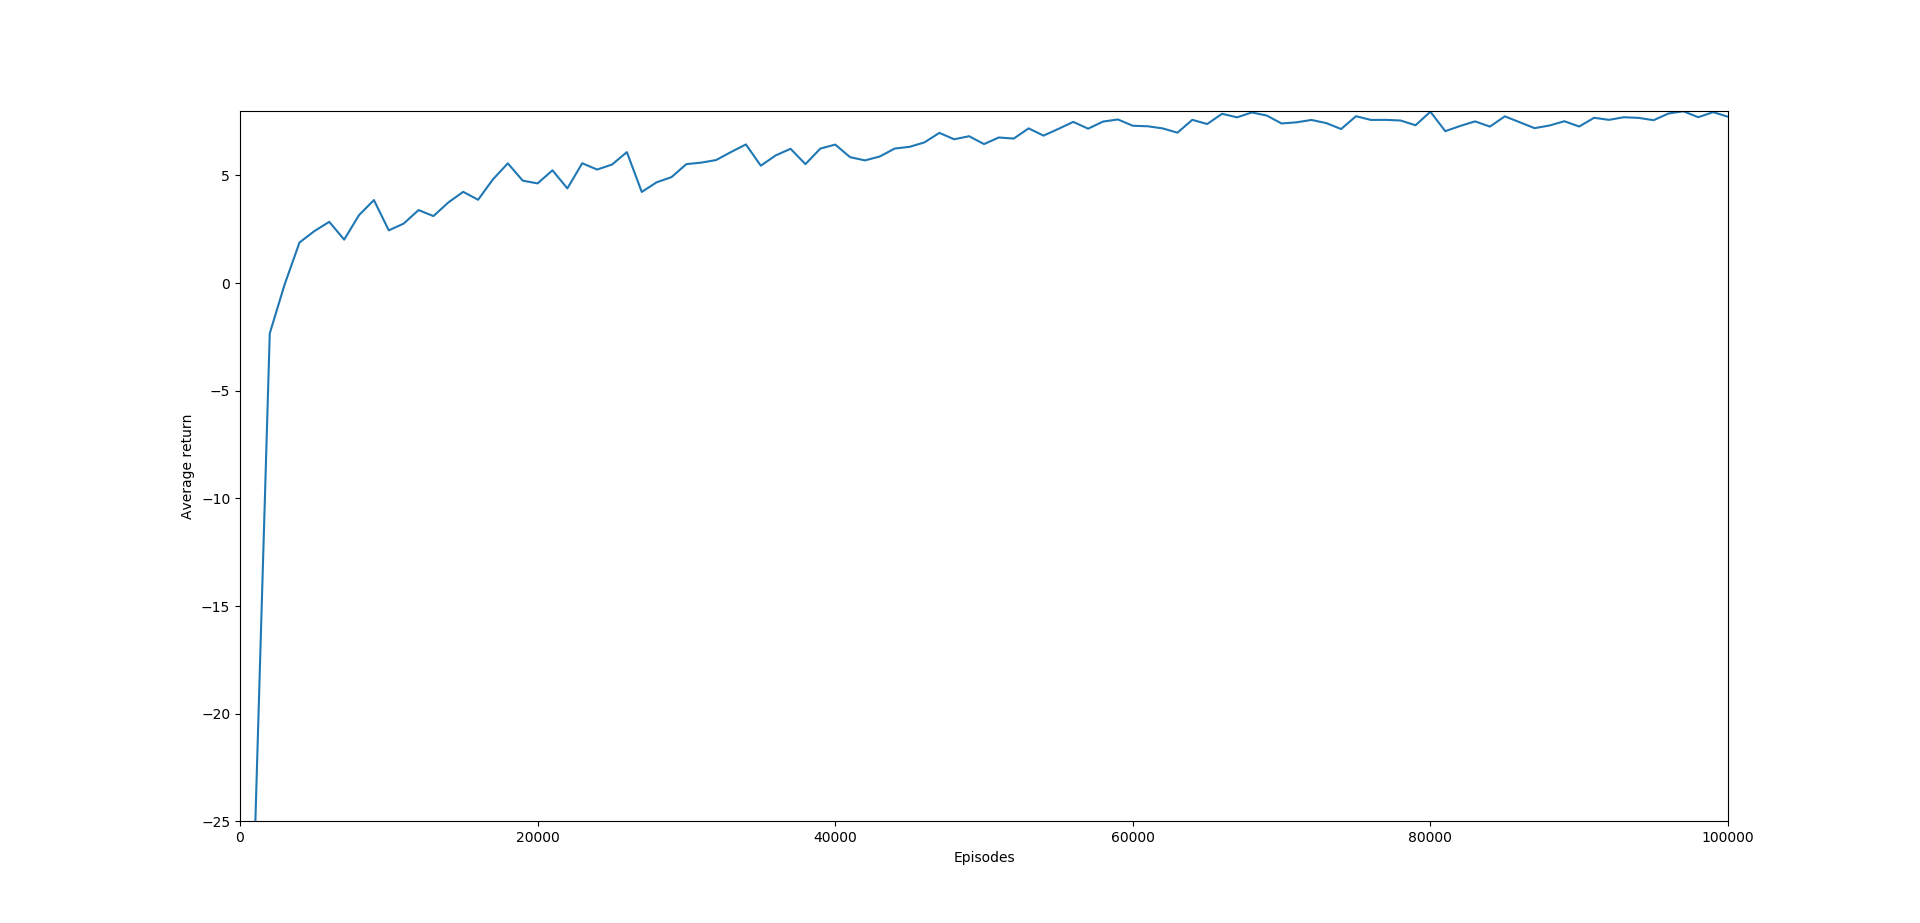
\includegraphics[width=0.7\linewidth]{p1.png}
\caption{training curve}
\label{fig:p1}
\end{figure}

\begin{figure}[!ht]
\centering
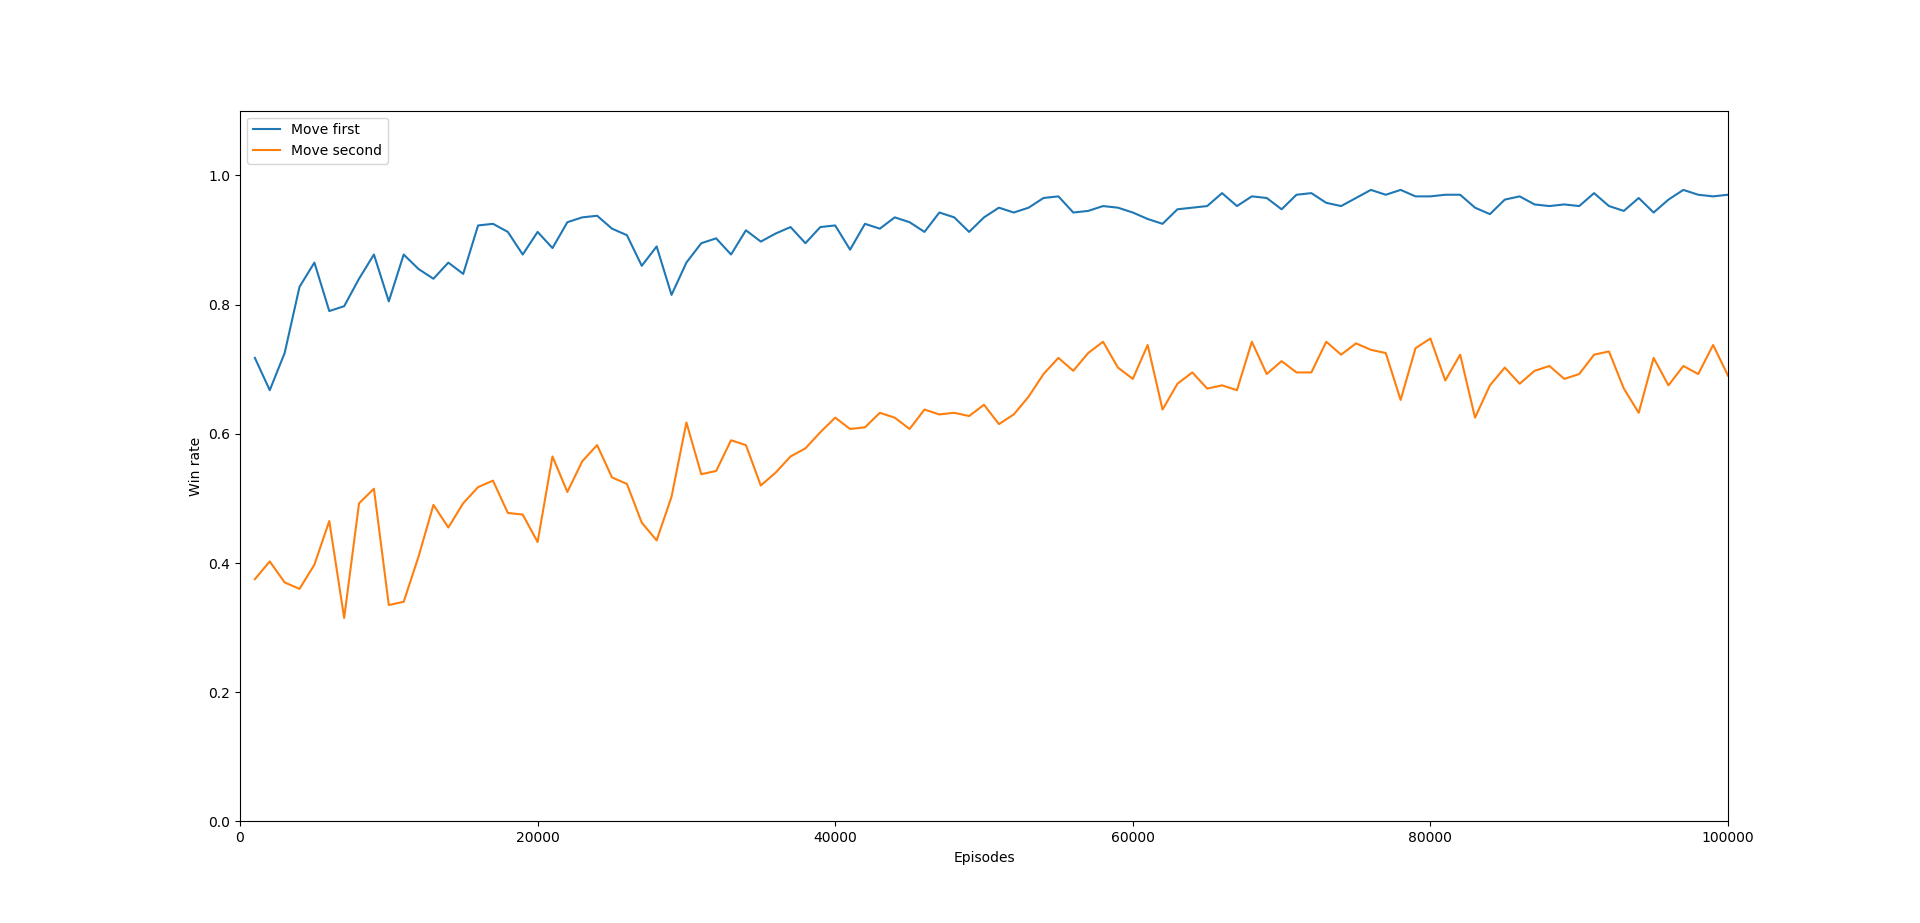
\includegraphics[width=0.7\linewidth]{p1winrate.png}
\caption{Winrate}
\label{fig:p1w}
\end{figure}

\begin{framed}
\begin{lstlisting}[language=python]
Policy plays first
===== Game1 =====
x..
...
...
====
x..
.o.
...
====
x..
xo.
...
====
xo.
xo.
...
====
xo.
xo.
x..
====
Learned policy wins against random! (learned policy moves first)

===== Game2 =====
x..
...
...
====
xo.
...
...
====
xo.
x..
...
====
xo.
x..
..o
====
xo.
x..
x.o
====
Learned policy wins against random! (learned policy moves first)


===== Game1 =====
x..
...
...
====
x..
o..
...
====
x..
o..
x..
====
x..
oo.
x..
====
x..
oox
x..
====
x..
oox
x.o
====
xx.
oox
x.o
====
xxo
oox
x.o
====
xxo
oox
xxo
====
Learned policy ties against random! (random moves first)

===== Game2 =====
x..
...
...
====
x..
o..
...
====
x..
o..
..x
====
x..
oo.
..x
====
x..
oox
..x
====
x.o
oox
..x
====
xxo
oox
..x
====
xxo
oox
.ox
====
xxo
oox
xox
====
Learned policy ties against random! (random moves first)

===== Game3 =====
x..
...
...
====
x..
o..
...
====
x..
o..
..x
====
x..
oo.
..x
====
x..
oox
..x
====
x.o
oox
..x
====
x.o
oox
.xx
====
x.o
oox
oxx
====
Learned policy wins against random! (random moves first)
\end{lstlisting}
\end{framed}

\end{homeworkProblem}
\clearpage
%----------------------------------------------------------------------------------------
%	PROBLEM 2
%----------------------------------------------------------------------------------------
\begin{homeworkProblem}
\noindent \textit{Self-play}\\
The winrate for both playing first and playing second doesn't really increase. In fact they seems to decrease a bit. So I use the weights at 60000 episode for testing\\
The graphs also include the win and tie rate because I feel like for tictactoe game, tie is inevitable some time.
\begin{figure}[!ht]
\centering
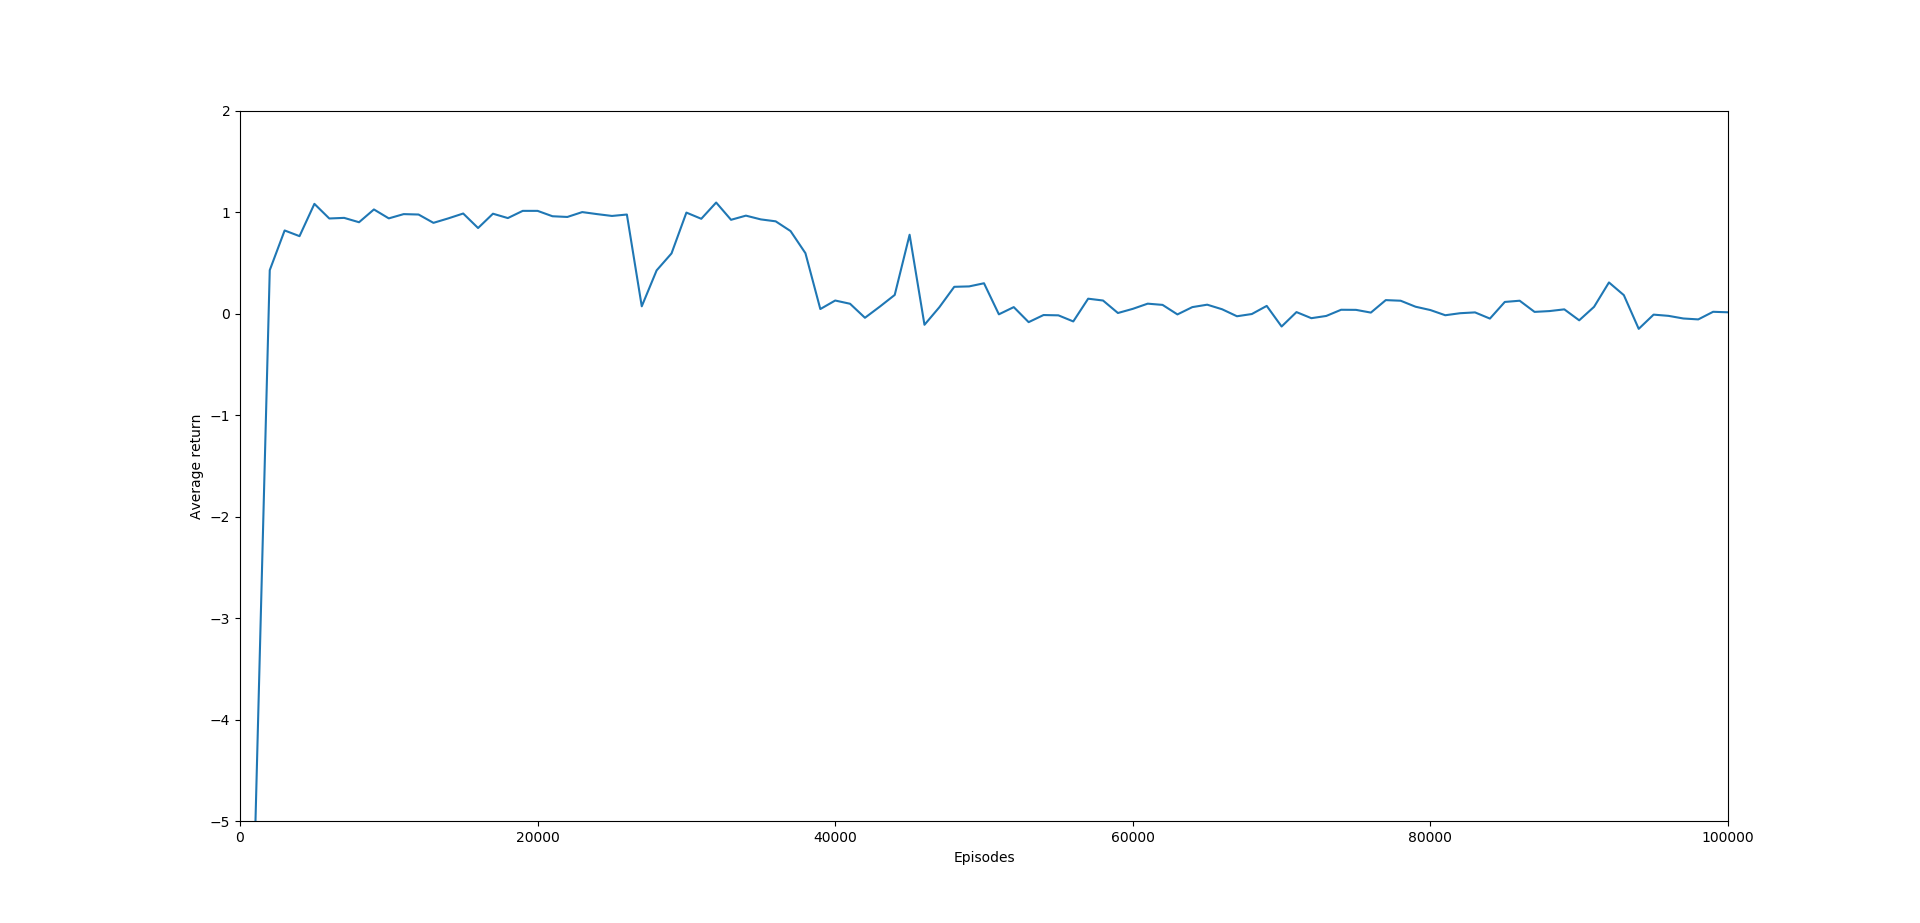
\includegraphics[width=0.9\linewidth]{p2.png}
\caption{Learning curve}
\label{fig:p2}
\end{figure}
\begin{figure}[!ht]
\centering
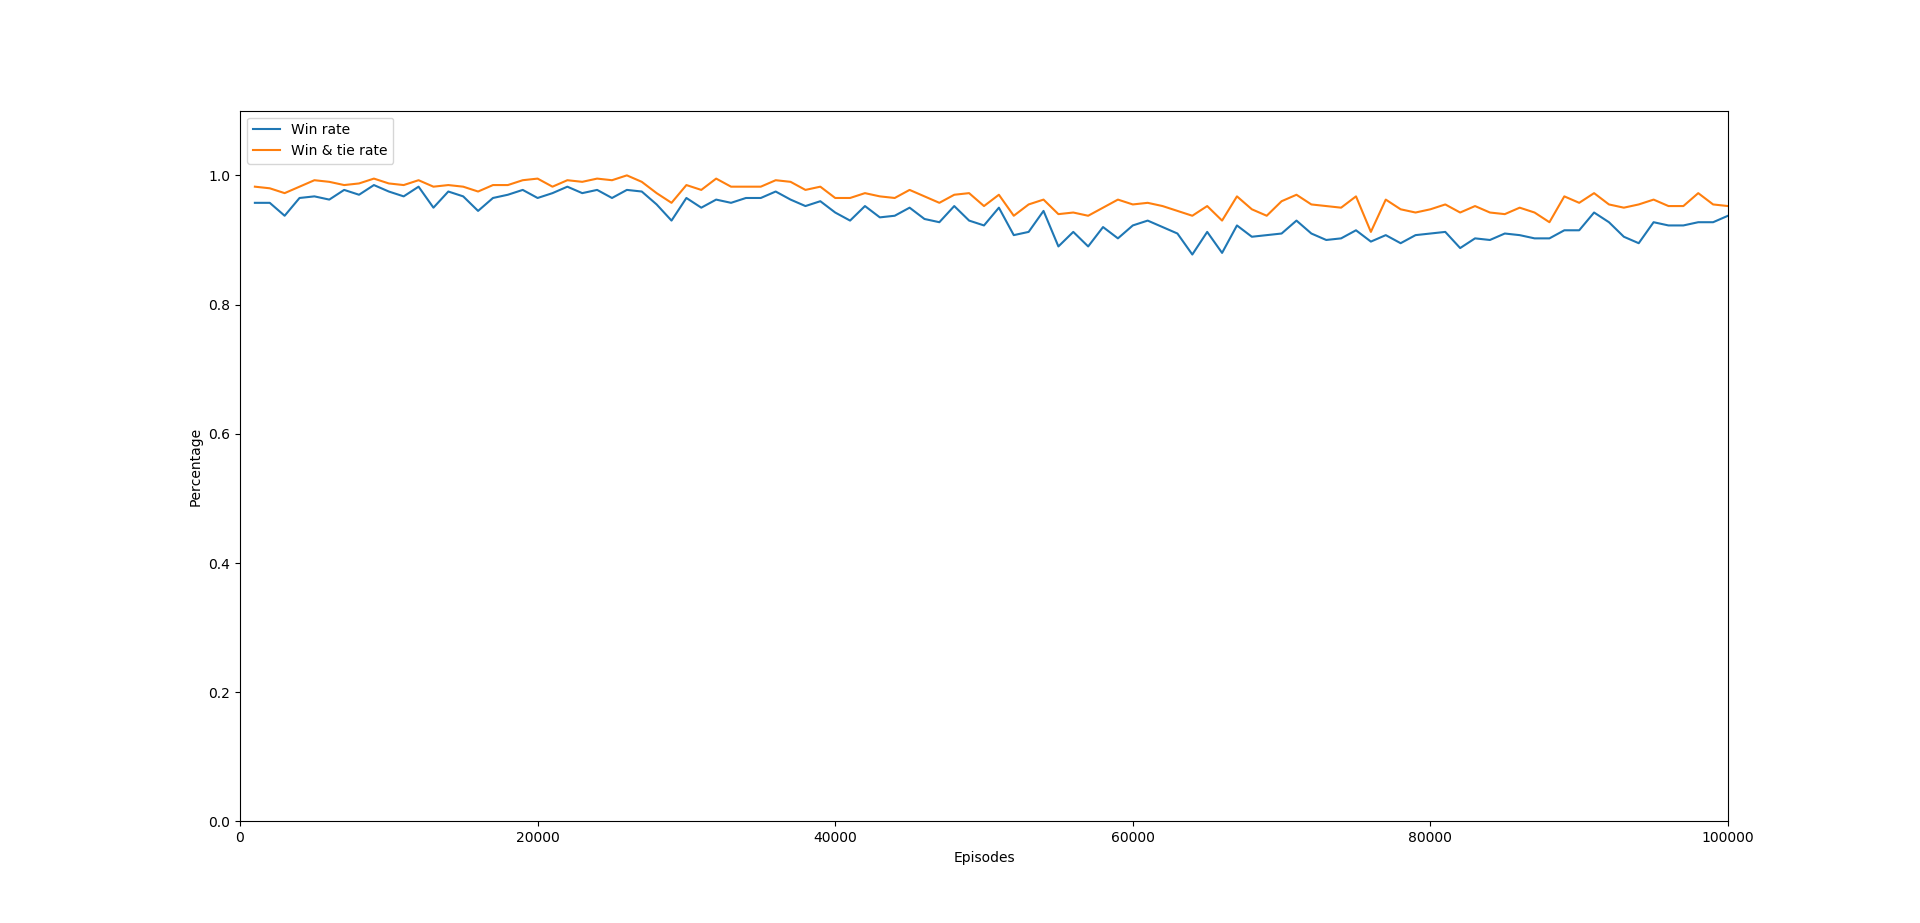
\includegraphics[width=0.9\linewidth]{p2wt1.png}
\caption{Win and tie rate for playing first for 400 games}
\label{fig:p2wt1}
\end{figure}
\begin{figure}[ht]
\centering
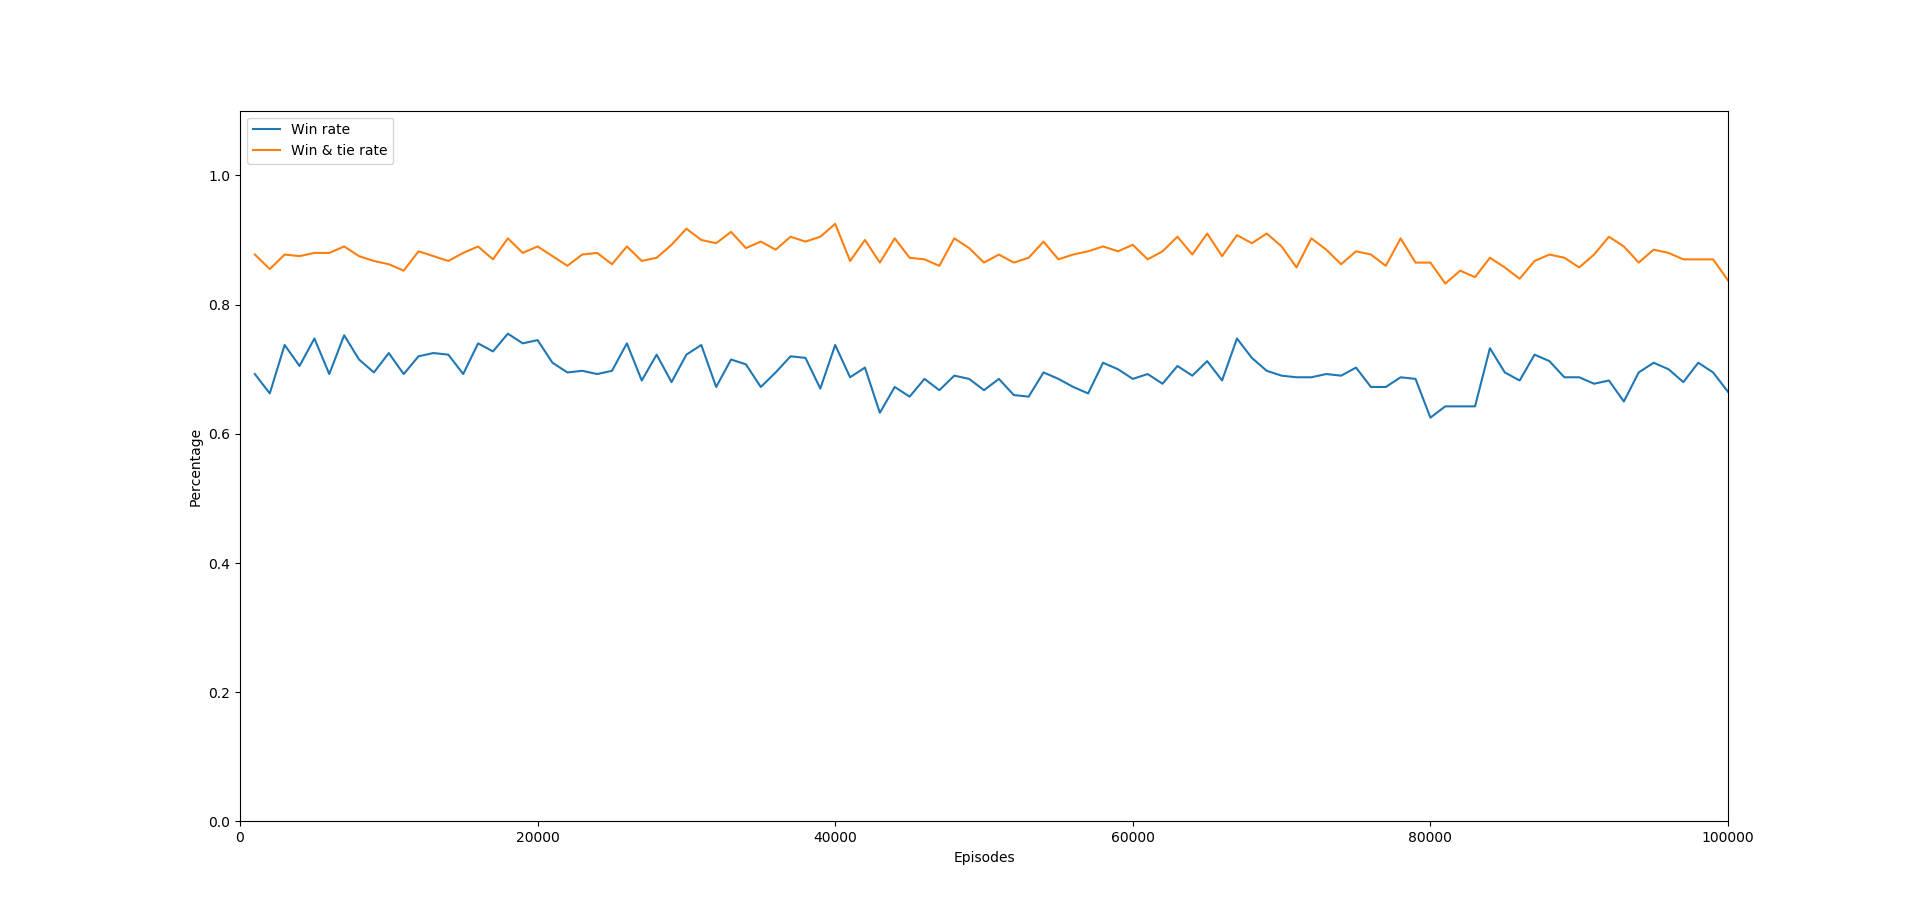
\includegraphics[width=0.9\linewidth]{p2wt2.png}
\caption{Win and tie rate for playing second for 400 games}
\label{fig:p2wt2}
\end{figure}
\\
\\
\\
\\
\\
\\
Against random player
\begin{framed}
\begin{lstlisting}[language=python]
===== Game1 =====
...
.x.
...
====
...
.xo
...
====
x..
.xo
...
====
x..
oxo
...
====
x..
oxo
..x
====
Learned policy wins against random! (learned policy moves first)

===== Game2 =====
...
.x.
...
====
.o.
.x.
...
====
xo.
.x.
...
====
xo.
.x.
.o.
====
xo.
.x.
xo.
====
xo.
ox.
xo.
====
xox
ox.
xo.
====
Learned policy wins against random! (learned policy moves first)

===== Game1 =====
...
.x.
...
====
o..
.x.
...
====
o..
.xx
...
====
o..
oxx
...
====
o..
oxx
..x
====
o..
oxx
o.x
====
Learned policy wins against random! (random moves first)

===== Game2 =====
...
.x.
...
====
o..
.x.
...
====
o..
.x.
..x
====
o..
ox.
..x
====
ox.
ox.
..x
====
ox.
ox.
o.x
====
Learned policy wins against random! (random moves first)

===== Game3 =====
...
.x.
...
====
o..
.x.
...
====
o..
.x.
x..
====
o.o
.x.
x..
====
o.o
.xx
x..
====
o.o
oxx
x..
====
oxo
oxx
x..
====
oxo
oxx
xo.
====
oxo
oxx
xox
====
Learned policy ties against random! (random moves first)
\end{lstlisting}
\end{framed}

Against self
\begin{framed}
\begin{lstlisting}[language=python]
===== Game1 =====
x..
...
...
====
x..
...
o..
====
x..
...
o.x
====
x..
.o.
o.x
====
x.x
.o.
o.x
====
xox
.o.
o.x
====
xox
.ox
o.x
====
First player wins!

===== Game2 =====
...
.x.
...
====
o..
.x.
...
====
o..
.x.
..x
====
o..
ox.
..x
====
o..
ox.
x.x
====
o..
ox.
xox
====
o.x
ox.
xox
====
First player wins!

===== Game3 =====
...
.x.
...
====
o..
.x.
...
====
o..
.x.
..x
====
o..
ox.
..x
====
o..
ox.
x.x
====
o..
ox.
xox
====
o.x
ox.
xox
====
First player wins!

===== Game4 =====
...
.x.
...
====
o..
.x.
...
====
o..
xx.
...
====
o..
xxo
...
====
o..
xxo
..x
====
o..
xxo
.ox
====
o..
xxo
xox
====
o.o
xxo
xox
====
oxo
xxo
xox
====
Tie.

===== Game5 =====
...
.x.
...
====
o..
.x.
...
====
o..
.x.
..x
====
o..
ox.
..x
====
o..
ox.
x.x
====
o..
ox.
xox
====
o.x
ox.
xox
====
First player wins!
\end{lstlisting}
\end{framed}
\end{homeworkProblem}
\clearpage


%----------------------------------------------------------------------------------------

\end{document}
